
\section{Обзор предметной области} % (fold)
\label{sec:domain}

% В данном разделе будет произведён обзор предметной области задачи, решаемой в рамках дипломного проекта;
% рассмотрены вопросы о сущности байесовых сетей и принципе их работы; приведена оценка сложности различных проблем, возникающих при применении вероятностных сетей для решения прикладных задач.
% Также будут рассмотрены принципы работы алгоритмов вывода структуры по данным, реализованных в программном обеспечении разработанном в рамках дипломного проекта, и произведено сравнение с существующим ПО для решения схожих задач.

\subsection{Интеллектуальная собственность}
\label{sub:domain:ip}
В новой бизнес-модели для полупроводниковой промышленности, процесс проектирования начинается с поставщиков интеллектуальной собственности, которые создают многоразовые
логические блоки(далее \textit{IP-блоки}) и виртуальные компоненты. Так как эти поставщики специализируются в производстве IP-блоков, то последние являются тщательно протестированными и опробованными. В дополнение, блоки проектируются с учетом простоты интеграции в различные системы (plug and play). Системные интеграторы затем покупают лицензию на использование блоков и разрабатывают новые архитектуры для ASIC(интегральных схем специального назначения, англ. \textit{application-specific integrated circuit}), FPGA(программируемых пользователем вентильных матриц, англ. \textit{field-programmable gate array}) или SoC(систем на кристалле, англ. \textit{system-on-a-chip}), комбинируя различные IP-блоки, полученные от разных поставщиков. Получившийся дизайн интегральной схемы(в случае ASIC-схем) затем посылается на завод для изготовления.
Различают 3 вида блоков~\cite{conterfeit_integrated_circuits}:

\begin{itemize}
  \item Программные IP-блоки(Soft IPs) -- представлены в виде RTL(register-transfer level) абстракций. Поскольку они описаны с помощью HDL(hardware description language) или схожего по уровню абстракции языка, то они представляют собой цифровые IP-блоки, которые являются процессо-инвариантными и могут быть использованы для gate-level синтеза. Программные блоки очень гибкие и могут быть легко перенесены из одной системы в другую. С другой стороны, этот вид блоков даёт очень мало информации(или не предоставляет вовсе) о временных характеристиках и параметрах энергопотребления.
  \item Физические IP-блоки(Hard IPs) -- блоки, специфицированные на физическом уровне реализации, обычно представленные в форме файлов с расширением Graphical Database System II(GDSII). Эти блоки обладают фиксированным расположением элементов и предсказуемыми временными характеристиками, энергопотреблением и занимаемой площадью. Их основной недостаток- жесткость дизайна(ограничены одним технологическим процессом) и отсутствие портативности. Этот вид блоков наиболее распространен в аналоговых и смешанных системах.
  \item Схемотехнические IP-блоки(Firm IPs) -- нечто среднее между программными и физическими блоками. Специфицируются на схемотехническом уровне без привязки к конкретной топологической реализации. Обычно предоставляются в форме готового списка соединений и более предсказуемы, чем программные блоки. Могут быть легко перенесены на различные технологические процессы и оптизированы для потребностей разрабатывающей стороны.
\end{itemize}


\subsection{Повторное использование и пиратство}
\label{page:domain:piracy}
В полупроводниковой промышленности наблюдаются значительные улучшения в производительности за счет принципа повторного использования. Поставщики IP-блоков постоянно трудятся над улучшением компонентов и их гибкости для использования в нескольких дизайнах. Недавний опрос, проведенный среди ведующих производителей интегральных схем показал, что почти 68\% кремниевых матриц содержит повторно используемые компоненты~\cite{design_and_verification_report_2013}. Идея свободно-распространяемых логических блоков также довольно распространена сейчас. В результате, дизайнеры и поставщики работают вместе, что способствует повышению производительности труда в производстве интегральных схем. Однако повторное использование IP-блоков делает пиратство серьезной проблемой. IP-блоки -- интеллктуальная собственность дизайнера. Как и с любым другим продуктом, эти блоки являются объектом авторских прав, патентов и торговых марок. Пиратство приводит к неправильному, и часто несанкционированному использованию IP-блоков. Проблема может принимать различные формы:

\begin{itemize}
  \item заявляя, что чужой компонент является твоей собственностью и/или продажа оного;
  \item использование IP-блоков вне рамок их лицензии, например использование IP-блоков с открытым исходным кодом в коммерчеких целях;
  \item неуплата денег за компонент;
\end{itemize}

Более сложная и серьезная проблема в пиратстве -- реверс-инжиниринг\\(reverse ingineering). Реверс-инжиниринг -- процесс извлечения информации из конечного устройства или программы с целью понять принцип его работы. Но, как это предусмотрено законом, реверс-инжиниринг является законным в определенной степени. Разрешено использовать обратное проектирование IP-блока  или дизайна в обучающих целях, для анализа или оценки копцепций и методов.

\subsubsection{Подходы для защиты авторских прав}
\label{page:domain:secure_approaches}

Существуют различные меры для защиты IP-блоков:

\begin{itemize}
\item Саморазрушение(self-destruction): для военного применения. Блоки, которые встраиваются в схемы, имеют специальные химические компоненты, которые разрушают блок при любой попытке вскрытия или реверс-инжиниринга.
\item обфускация: структура и функциональность блока скрывается~\cite{obfuscation_soc_design} различными методами, такими как изменение структуры/содержания HDL компонентов для усложнения реверс-инжиниринга~\cite{obf_as_int_rights_prot_in_vhdl} или вставки конечных автоматов  в блок, которые не позволяют блоку нормально функционировать до тех пор, пока они не активированы правильной последовательностью~\cite{rtl_hardware_ip_protection};
\item Периодическое лицензирование: Таймеры и контроллеры лицензии встраиваются в IP-блок и позволяют следить за лицензионным периодом. Когда он заканчивается, IP-блок перестаёт работать.
\item шифрование: Потоки данных в FPGA схемах тщательно шифруются с помощью сильного алгоритма шифрования и ключ шифрования хранится в безопасности для предотвращения реверс-инжиниринга IP-блоков;
\end{itemize}

\subsection{Обфускация}
\label{page:domain:obfucation}
Обфускация -- широко известная методика защиты исходных кодов программ от обратного проектирования~\cite{collberg}. Основной её целью является затруднение понимания функционирования программы. В идеале, временные затраты и сложность реверс-инжиниринга должны оказаться близки к затратам на разработку системы с нуля~\cite{sergeichik_ivaniuk}.
Эта техника часто используется совместно с другими методами защиты от пиратства.\\
Существует большое число методов обфускации для различных языков программирования. Однако почти все эти методы неэффективны в случае VHDL, так как результаты применения обфускации никак не влияют на конечный результат синтеза, т.е схемы устройств до и после обфускации выглядят одинаково. Поэтому, в случае языка VHDL, следует рассматривать еще один вид обфускации -- функциональную~\cite{ivaniuk}.

\subsubsection{Лексическая обфускация}
\label{page:domain:lexical}

Лексическую обфускацию для языка VHDL можно представить как

\begin{equation}
  <V> = \{T;S;D;K\} \text{\,,}
  \label{eq:domain:lexical:view}
\end{equation}
\begin{explanation}
  где $T$-- множество терминалов; $S$-- множество выражений; $D$-- множество\\ объявлений; $K$-- множество комментариев.
\end{explanation}
Схему цифрового устройства $S_{ch}$ можно описать следующим образом~\cite{ivaniuk}:
\begin{equation}
  S_{ch}= \{IP;OP;B;L\} \text{\,,}
  \label{eq:domain:lexical:schema}
\end{equation}
\begin{explanation}
  где $IP$ -- множество входных портов; $OP$ -- множество выходных портов;\\$B$ -- множество функциональных блоков, из которых состоит схема\\ устройства; $L$ -- множество проводящих линий, соединяющих внутренние\\ блоки и порты.
\end{explanation}

Синтезом называется процесс интерпретации описания на языка V в схему:
\begin{equation}
  DD(V) = DD(\{T;S;D;K\}) = \{IP;OP;B;L\} = S_{ch}
  \label{eq:domain:lexical:synthesis}
\end{equation}
Тогда лексическим эквивалентным преобразованием будет называться замена одного фрагмента кода $V_1 = \{T;S;D;K\}$, результат синтеза которого
\begin{equation}
  DD(V_1) = DD(\{T;S;D;K\}) = \{IP;OP;B;L\} = S_{ch_1}\text{\,,}
  \label{eq:domain:lexical:equantinal_transform}
\end{equation}
другим фрагментом
\begin{equation}
  V_2 = \{T';S';D';K'\} \text{\,,}
  \label{eq:domain:lexical:equation_second}
\end{equation}
\begin{explanation}
  где $V_1 \neq V_2$, результат синтеза которого идентичен предыдущему:
\end{explanation}
\begin{equation}
  DD(V_2) = DD(\{T';S';D';K'\}) = \{IP;OP;B;L\} = S_{ch} = DD(V_1)
  \label{eq:domain:lexical:final_synth_equation}
\end{equation}

Сложность описания можно представить как функцию, зависящую от внутренней структуры $V$:
\begin{equation}
  C(V) = C(\{T';S';D';K'\}).
  \label{eq:domain:lexical:final_synth_equation}
\end{equation}

Лексическое обфусцирующее преобразование -- это лексическое эквивалентное преобразование, для которого дополнительно выполняется свойство <<сложность результирующего фрагмента $V_2$ больше, чем сложность исходного $V_1$>>:
\begin{equation}
  C(V_2) > V(V_1), DD(V_2) = DD(V_1).
  \label{eq:domain:lexical:final_synth_equation}
\end{equation}
\subsubsection{Виды лексических преобразований}

Существуют различные обфусционные преобразования, которые можно применить к VHDL:
\begin{itemize}
\item Замена имен переменных. Одна из самых простых трансформаций. Не влияет на результат синтеза и скорость, однако очень затрудняет чтение исходного кода злоумышленником.
\begin{figure}[ht]
\centering
  \begin{subfigure}[b]{0.45\textwidth}
    \centering
    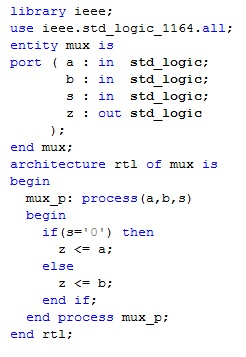
\includegraphics[scale=0.7]{variable_names_before.jpg}
    \caption*{ до обфускации }
  \end{subfigure}
  \begin{subfigure}[b]{0.45\textwidth}
    \centering
    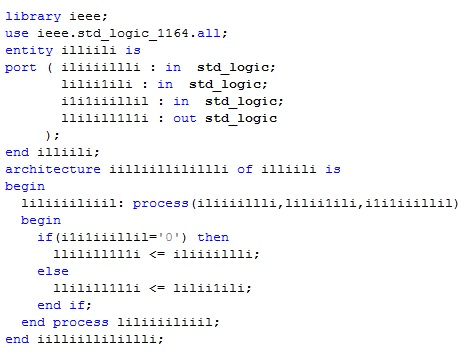
\includegraphics[scale=0.7]{variable_names_after.jpg}
    \caption*{ после обфускации }
  \end{subfigure}
  \caption{ Проектное описание до и после обфускации }
  \label{fig:fire_alarms}
\end{figure}

\item Встраиваемые функции. Часть кода выносится в отдельную функцию, а сам код заменяется вызовом этой функции. Результат синтеза остаётся тем же, злоумышленнику сложнее отследить потоки данных в исходном коде программы.


\begin{figure}[ht]
\centering
  \begin{subfigure}[b]{0.45\textwidth}
    \centering
    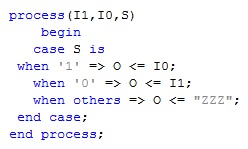
\includegraphics[scale=0.7]{inlining_before.jpg}
    \caption*{до обфускации}
  \end{subfigure}
  \begin{subfigure}[b]{0.45\textwidth}
    \centering
    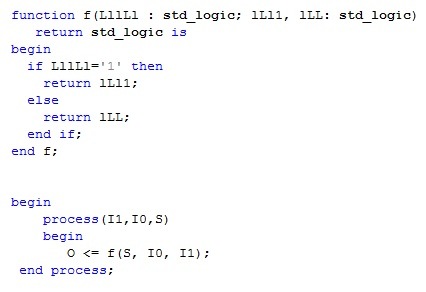
\includegraphics[scale=0.7]{inlining_after.jpg}
    \caption*{после обфускации}
  \end{subfigure}
  \caption{ Проектное описание до и после обфускации }
  \label{fig:fire_alarms}
\end{figure}

\item Фиктивные выражения(bogus statements). В код добавляются выражения, не несущие никакого  логического смысла, однако затрудняют понимание кода злоумышленником.


\begin{figure}[ht]
\centering
  \begin{subfigure}[b]{0.45\textwidth}
    \centering
    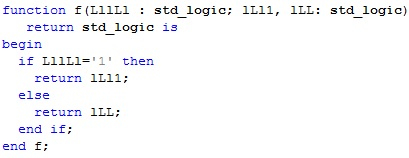
\includegraphics[scale=0.65]{bogus_before.jpg}
    \caption*{до обфускации}
  \end{subfigure}
  \begin{subfigure}[b]{0.45\textwidth}
    \centering
    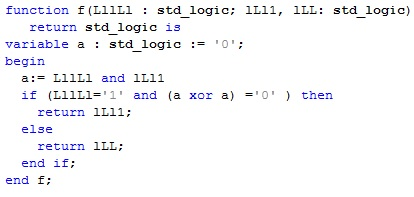
\includegraphics[scale=0.7]{bogus_after.jpg}
    \caption*{после обфускации}
  \end{subfigure}
  \caption{ Проектное описание до и после обфускации }
  \label{fig:fire_alarms}
\end{figure}


\item Дублирование кода. В код вставляются одинаковые по логике, однако внешне разные по виду фрагменты кода.


\begin{figure}[ht]
\centering
  \begin{subfigure}[b]{0.45\textwidth}
    \centering
    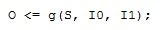
\includegraphics[scale=0.7]{dup_before.jpg}
    \caption*{до обфускации}
  \end{subfigure}
  \begin{subfigure}[b]{0.45\textwidth}
    \centering
    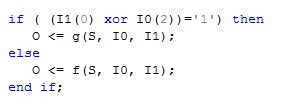
\includegraphics[scale=0.7]{dup_after.jpg}
    \caption*{после обфускации}
  \end{subfigure}
  \caption{ Проектное описание до и после обфускации}
  \label{fig:fire_alarms}
\end{figure}

\end{itemize}

Также существуют другие типы лексических преобразований:
\begin{itemize}
\item Добавление нового уровня интерпретации. Определяется собственный набор инструкций, программа переводится на новый набор инструкций, пишется интерпретатор для данного набора инструкций. Как результат, программа станровится в 10-100 раз медленнее.
\item Chengxification. Представляет собой разворачивание потока управления программы. Каждый оператор помещается внутрь условной конструкции switch и выполняется при определенном условии.
\end{itemize}
Однако, в силу специфики языка, эти методы плохо применимы(или неприменимы вовсе) к VHDL.

\subsubsection{Функциональная обфускация}

Функциональность устройства $Sch$ можно определить как зависимость значений на выходных портах $OP$ от значений на входных портах $IP$, внутренних блоков $B$ и проводящих линий $L$~\cite{ivaniuk}:

\begin{equation}
  OP = F_{Sch} (IP;B;L) \text{\,.}
  \label{eq:domain:functional:basis}
\end{equation}

Пусть существует другое устройство $Sch'$, схема которого описывается выражением

\begin{equation}
  Sch' = \{IP;OP;B';L'\} \text{\,,}
  \label{eq:domain:lexical:schema}
\end{equation}
при этом множество блоков $B'$ и множество линий $L'$ не совпадают с аналогичными множествами устройства $Sch$.

Устройства $Sch$ и $Sch'$ будут функционально эквивалентными, если выполняется следующее равенство~\cite{ivaniuk}:
\begin{equation}
  F_{Sch}(IP;B;L) = F_{Sch'}(IP;B';L') \text{\,.}
  \label{eq:domain:functional:basis}
\end{equation}

Функционально эквивалентное преобразование - это замена одного фрагмента кода $V_1 = \{T;S;D;K\}$, результат синтеза которого
\begin{equation}
  DD(V_1) = DD(\{T;S;D;K\}) = \{IP;OP;B;L\} = S_{ch_1} \text{\,,}
  \label{eq:domain:functional:schema}
\end{equation}
другим фрагментом $V_2 = \{T';S';D';K'\}$, результат синтеза которого
\begin{equation}
  DD(V_2) = DD(\{T';S';D';K'\}) = \{IP;OP;B';L'\} = S_{ch_2} \text{\,.}
  \label{eq:domain:functional:schema}
\end{equation}

При этом $Sch_2$ не совпадает с $Sch_1$. Однако наблюдаемое поведение~\cite{collberg} обеих схем идентично.

Тогда преобразование функциональной обфускации - это функциональное эквивалентное преобразование, для которого дополнительно выполняется свойство <<сложность результирующей схемы $Sch_2$ выше, чем сложность исходной $Sch_1$>>:

\begin{equation}
  C_{Sch_1}(IP;OP;B;L) = C_{Sch_2}(IP;OP;B';L') \text{\,.}
  \label{eq:domain:functional:schema}
\end{equation}

\subsubsection{Генераторы константных значений}

Множество функциональных обфусцирующих преобразований основывается на генераторах константных значений. Проблема состоит в том, чтобы избежать упрощения схемы. Ниже приведены примеры реализации генераторов константных значений и результат их синтеза. На основе этих элементов можно производить преобразования базовых вентилей. Примером функциональной обфускации может быть мультиплексор, первый вход которого подключен к константе 0. С помощью некоторых ухищрений можно добиться того, что синтезатор не распознает в данной схеме and.


\begin{figure}[ht]
\centering
  \begin{subfigure}[b]{1\textwidth}
    \centering
    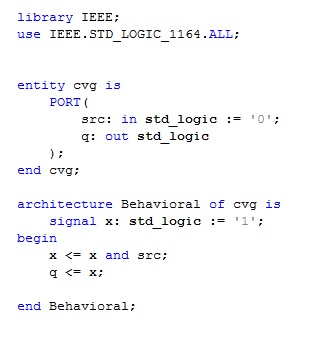
\includegraphics[scale=1]{cvg_code_1.jpg}
    \caption*{исходный код}
  \end{subfigure}
  \begin{subfigure}[b]{1\textwidth}
    \centering
    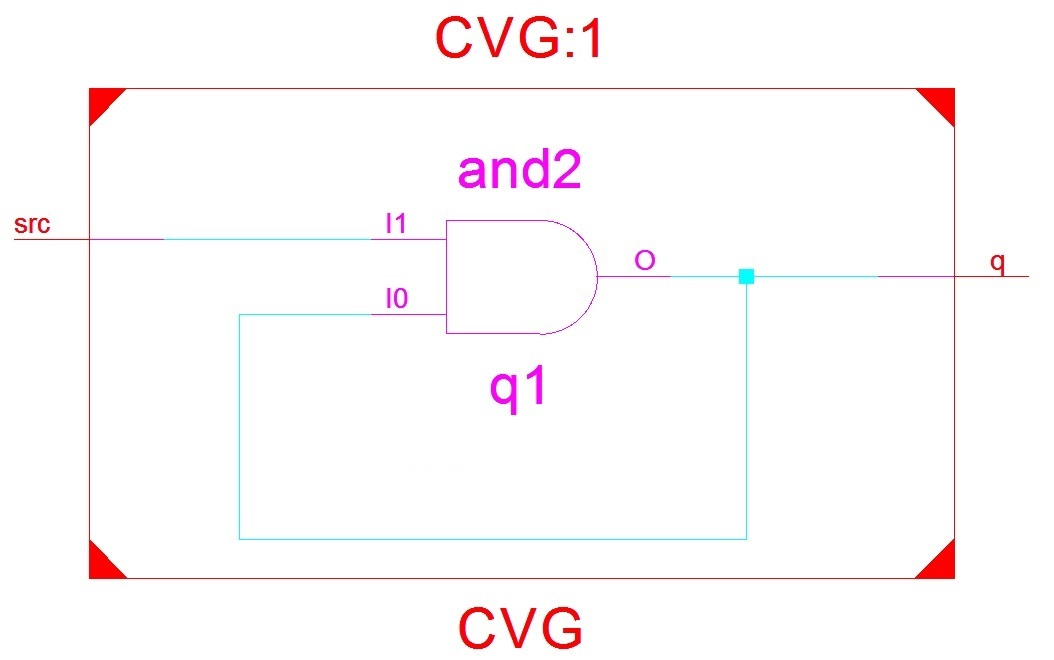
\includegraphics[scale=0.5]{cvg_scheme_inverted_1.jpg}
    \caption*{результат синтеза}
  \end{subfigure}
  \caption{ Генератор константных значений с использованием комбинационной логики}
  \label{fig:fire_alarms}
\end{figure}



\begin{figure}[ht]
\centering
  \begin{subfigure}[b]{1\textwidth}
    \centering
    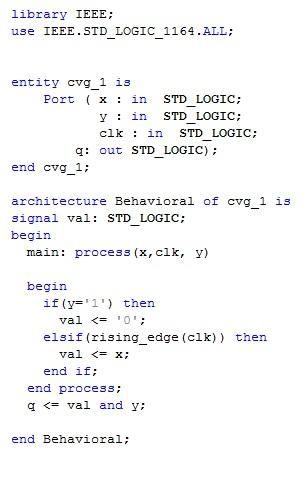
\includegraphics[scale=1]{cvg_code_2.jpg}
    \caption*{исходный код}
  \end{subfigure}
  \begin{subfigure}[b]{1\textwidth}
    \centering
    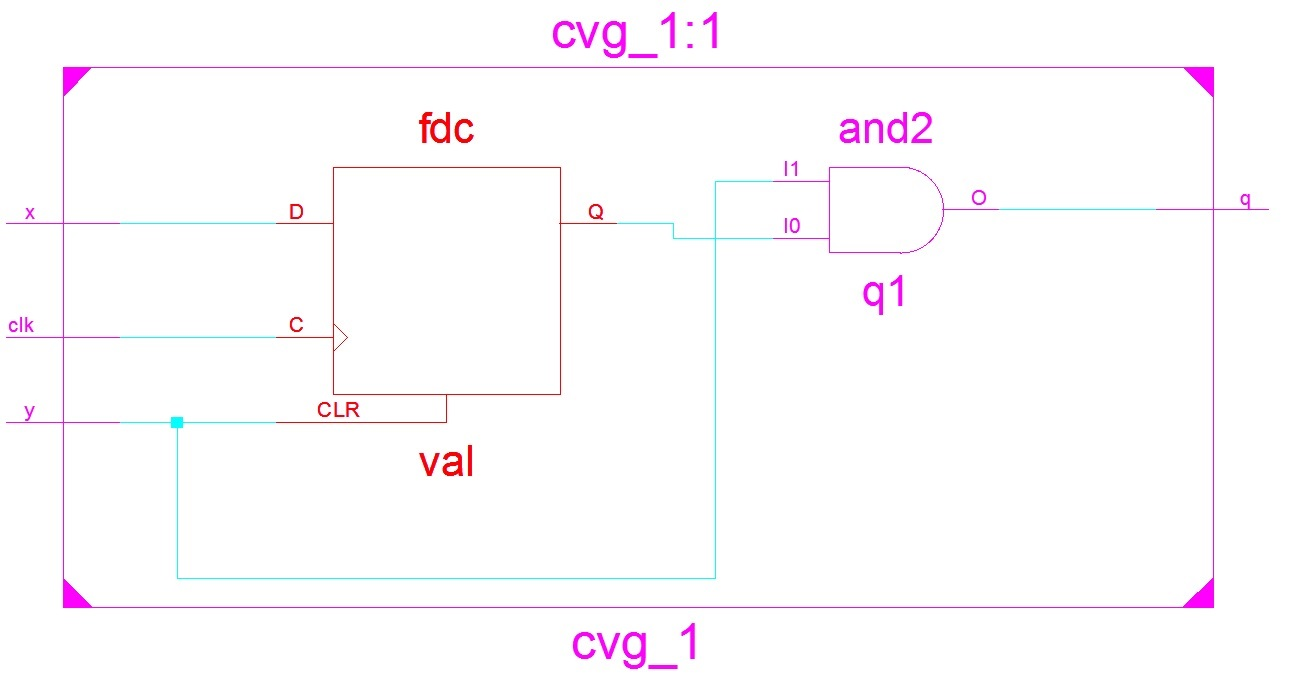
\includegraphics[scale=0.5]{cvg_scheme_inverted_2.jpg}
    \caption*{результат синтеза}
  \end{subfigure}
  \caption{ Генератор константных значений с элементом памяти }
  \label{fig:fire_alarms}
\end{figure}





\begin{figure}[ht]
\centering
  \begin{subfigure}[p]{1\textwidth}
    \centering
    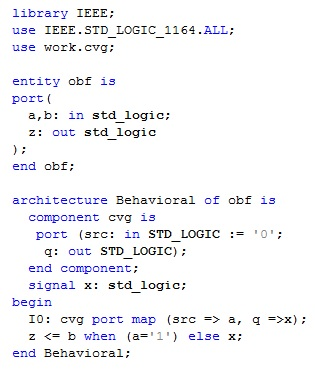
\includegraphics[scale=1]{obfand_code.jpg}
    \caption*{исходный код}
  \end{subfigure}
  \begin{subfigure}[b]{1\textwidth}
    \centering
    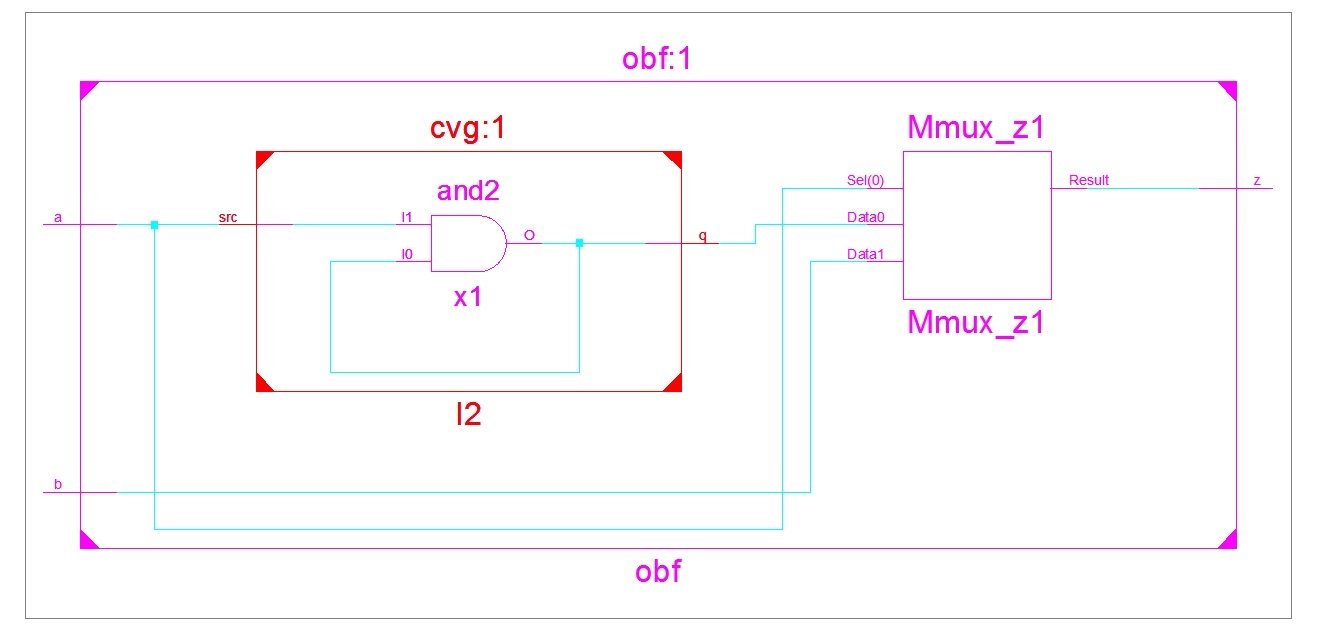
\includegraphics[scale=0.5]{obfand_scheme.jpg}
    \caption*{результат синтеза}
  \end{subfigure}
  \caption{ Обфусцированный вентиль and }
  \label{fig:fire_alarms}
\end{figure}

\FloatBarrier


\subsubsection{Временные характеристики}

Поскольку результатом работы исходного кода, написанного на языке VHDL, является синтезированная схема, то увеличение сложности может сопровождаться дополнительными потерями в энергопотреблении и скорости работы схемы. В случае лексической обфускации этого не происходит, так как оная никак не влияет на результат синтеза. Однако использование функциональной(в частности применение генераторов константных значений) может существенно замедлить работу схемы. В тех случаях, когда скорость работы является критичной, необходимо или отказываться от использования функциональной обфускации, или балансировать между производительностью и уровнем сложности схемы. Дополнительные манипуляции, такие как избегание использования данных генераторов на критических путях схемы, помогают избегать дополнительных расходов в производительности. В таблице \ref{table:domain:overheads}
приведены накладные расходы при использовании генераторов константных значений. Для тестов использовались эталонные схемы ISCAS 99~\cite{iscas}. В качестве контрольных наборов использовались генераторы числом 1,3,5 на различных схемах. Использовался сбалансированный режим оптимизации. Значения, представленные в таблице отражают процент задержки в скорости работы схем при использовании оных.


\begin{longtable}[l]{| >{\centering}m{0.10\textwidth}
                  | >{\centering}m{0.175\textwidth}
                  | >{\centering}m{0.175\textwidth}
                  | >{\centering}m{0.175\textwidth}
                  | >{\centering\arraybackslash}m{0.175\textwidth}|}

  \caption{Накладные расходы при использовании генераторов константных значений}
  \label{table:domain:overheads}\tabularnewline
  \hline
         \multirow{2}{0.10\textwidth}[-0.5em]{\centering Схема}
       & \multicolumn{4}{c|}{\centering Количество генераторов} \tabularnewline
  \cline{2-5} & { 0 }  & { 1 }  & { 3 }   & { 5 } \tabularnewline


    % Схема & Без генератора & 1 Генератор & 3 Генератора & 5 Генераторов \\
   \hline
   b01 & 0\% & -52\% & -113\% & - 116\% \\
   \hline
   b07 & 0\% & -51\% & -85\% &  -85\% \\
   \hline
   b10 & 0\% & -33\% & -59\% & -20\% \\
   \hline
   b12 & 0\% & -18\% & -6\% & -1\% \\
   \hline
   b14 & 0\% & -29\% & -41\% & -41\% \\
   \hline
   b16 & 0\% & -11\% & 5\% & 1\% \\
   \hline
   b18\_1 & 0\% & 5\% & -3\% & 1\% \\
   \hline
   b20 & 0\% & 1\% & -11\% & 6\% \\
   \hline
   b22\_1 & 0\% & -3\% & 1\% & -1\% \\
   \hline

\end{longtable}

Как видно из таблицы \ref{table:domain:overheads}, результаты задержек, полученные из отчета синтезатора являются неприемлемо высокими. При увеличении сложности схемы, задержки, вызываемые добавлением генератора становятся менее значительными. При увеличении количества генераторов последующее добавление оных имеет всё меньшее влияние на временные характеристики. Это можно заметить, если сравнить задержки в более сложных схемах при использовании 3 и 5 генераторов. Фактическая задержка, вызываемая одним генератором, составляет примерно 0.3ns(наносекунд), что может критично сказываться на небольших схемах, но при этом может с успехом использоваться в более сложных. Однако, следует помнить, что задержка, вызываемая увеличением сложности не является константным значениеми можем варьироваться в зависимости от многих факторов:
\begin{itemize}
\item коэффицент объединения по входу/выходу элемента, к которому подключен генератор;
\item нахождение генератора на критическом пути;
\item логика, в которой генератор принимает участие(теоретически, возможно даже получить увеличение быстродействия);
\end{itemize}

\subsection{Обзор существующих аналогов}

Техники и алгоритмы, описанные выше, уже реализованы в программных продуктах фирм xilinx и aldec~\cite{aldec_obf}, однако, поскольку эти продукты являются закрытыми и не могут быть запущены вне этого программного комплекса, то сравнительный анализ данного программного средства с оными невозможен. Исходя из отсутствия свободно распространяемых утилит по обфускации проектных описаний цифровых устройств, разработка данного программного средства имеет смысл.
% \begin{explanation}


\subsection{Постановка задачи}
В результате выполнения дипломного проекта должно быть разработано программное средство лексической и функциональной обфускации проектных описаний цифровых устройств, описанных на языке VHDL со следующими спецификациями:
\begin{itemize}
\item разрабатываемое ПО должно иметь возможность запускаться под платформами Windows(7,8,10) и Linux(Ubuntu, Arch Linux, Linux Mint);
\item ПО работает в совокупности с другими средствами описания аппаратуры интегральных схем и должно иметь возможность запускаться в форме скрипта;
\item разрабатываемое ПО должно позволять производить только лексическую(или только функциональную) обфускацию в зависимости от требований конечного пользователя;
\end{itemize}
